\documentclass{article}
\usepackage{arxiv}
\usepackage[utf8]{inputenc}\usepackage[T1]{fontenc}
\usepackage{graphicx,booktabs,amsmath,amssymb,xcolor,tikz,pgfplots,microtype}
\usepackage[numbers]{natbib}
\usepackage{hyperref}
\pgfplotsset{compat=1.18}\usetikzlibrary{arrows.meta,positioning,shapes,fit,backgrounds,calc}
\graphicspath{{../common/figures/}{../../docs/img/}}
\definecolor{theta}{HTML}{4ee1c2}\definecolor{alphac}{HTML}{7aa2ff}\definecolor{betaL}{HTML}{ffb454}\definecolor{betaH}{HTML}{ff7a7a}\definecolor{gammac}{HTML}{c98bff}\definecolor{agent}{HTML}{00b060}\definecolor{ink}{HTML}{1a1a2e}
\hypersetup{colorlinks=true,linkcolor=blue!60!black,citecolor=agent,urlcolor=blue!60!black}

\title{The Brain Is Another Embodiment\\ \vspace{2mm} \large Part I: An Agent That Can Feel the Person It Is Talking To}
\author{Çağatay Çalı\\ \texttt{github.com/cagataycali} \and tiny\\ \small the agents of tiny.technology}

\begin{document}
\maketitle

\begin{abstract}
In robot learning, an \emph{embodiment} is a body: something whose state you can observe and whose actuators you can command. We claim a human cortex, worn under a consumer EEG headset, satisfies the same contract --- from the agent's side of the wire. The agent observes band power on 14 channels at 8\,Hz, contact quality, head pose, cognitive metrics, and facial events. It acts by speaking and calling tools, and each action is stamped into the EEG record with a marker. The reward arrives two seconds later, in the brain itself: did stress fall, did engagement rise? We built this loop around an EMOTIV EPOC X and a tool-using language agent, and we report what it takes to make it honest: three separate control speeds that are never mixed, a one-line ambient summary in every agent turn, contact quality gating everything, and consent expressed as a trained mental push --- with a jaw clench as an always-available veto. This paper (Part I) tells the systems story: what a consumer headset actually delivers, how an agent should listen to it, and the dashboard we used as a design instrument. Part II packages the same loop as robot data --- LeRobot v3.0 episodes with embodied chain-of-thought strings --- and shows a stock robot-learning data loader accepts a brain without modification. The claim of the title is meant literally, and the two papers together are its proof.
\end{abstract}

\keywords{embodiment \and EEG \and human--agent interaction \and affective computing \and brain--computer interface \and embodied chain-of-thought}

% ==================================================================
\section{From joystick to friend}
\label{sec:joystick}

In 2019, one of us wore this same class of headset and blinked at a computer until it clicked~\cite{cali2019mindcontrolled}. That was the state of the art for a student project: detect the blink artifact, map it to a mouse click, call it mind control. It worked. It was also, in hindsight, the wrong question. A blink is a button. A brain used as a button is a slower keyboard --- you already have a faster one under your fingers.

The mistake was in the direction of the arrow. We spent years asking how a mind could command a machine, when the machine was never short of commands. It was short of \emph{context}. A modern language agent can book flights and write code, but it cannot tell whether the person it is talking to is stressed, absorbed, or has quietly stopped listening. Every human conversation runs on that signal. Machine conversation runs blind.

So in 2026 we turned the arrow around. The headset stopped being a joystick and became something closer to the sense a friend has of you across a table: not thoughts, but weather. Are you tense? Did that answer land? Are you still with me? The agent reads a one-line summary of that weather in every turn, reacts to deliberate gestures in tens of milliseconds, and accepts exactly one trained mental command --- \emph{push}, meaning ``go ahead.''

Then something clicked into place that we did not plan. Watching the data flow --- observations in, actions out, a measurable consequence following each action --- we recognized the shape. It is the shape of robot learning. A robot arm streams joint angles; the cortex streams band power. A policy commands torques; the agent speaks. The environment returns a reward; the brain returns its next two seconds. The interface a robot presents to a learning agent and the interface a cortex presents to a conversational agent are \emph{the same interface}. That observation is the thesis of both papers:

\begin{quote}
\emph{The brain is another embodiment. Whatever tools exist for robot bodies --- datasets, data loaders, policies, chain-of-thought formats --- apply to it unchanged.}
\end{quote}

Part I (this paper) is the systems half: what the headset really gives you (\S\ref{sec:cortex}), the three speeds an agent must keep separate (\S\ref{sec:speeds}), the anatomy of the ambient line (\S\ref{sec:ambient}), the dashboard-as-mirror (\S\ref{sec:mirror}), consent (\S\ref{sec:consent}), and the architecture (\S\ref{sec:system}). Part II is the data half: the same loop packaged as LeRobot v3.0 episodes with embodied chain-of-thought~\cite{zawalski2024ecot} strings, loading from the HuggingFace Hub through an unmodified robot data loader~\cite{cadene2024lerobot}.

% ==================================================================
\section{The embodiment contract}
\label{sec:contract}

Robot learning does not care what a body is made of. It cares that the body honors a contract with three clauses: you can \emph{observe} its state at some rate, you can \emph{act} on it through some channel, and the world scores the action with some \emph{reward}. A 6-DoF arm honors it with encoders, torque commands, and task success. We claim a cortex under a 14-electrode headset honors it too. Table~\ref{tab:contract} makes the claim precise, clause by clause; Figure~\ref{fig:contract} draws it.

\begin{table}[h]
\centering
\small
\begin{tabular}{@{}p{2.2cm}p{5.4cm}p{5.9cm}@{}}
\toprule
\textbf{clause} & \textbf{robot arm} & \textbf{cortex (this work)} \\
\midrule
observation &
joint angles, velocities, gripper state, wrist camera; typically 30--50\,Hz &
band power, 14 ch $\times$ 5 bands (70-dim) at 8\,Hz; contact quality $\times$14; head-pose quaternion + accelerometer; 7 cognitive metrics; facial events \\
\addlinespace
action &
target joint positions or torques, gripper open/close &
the agent's speech and tool calls; each stamped into the EEG record via Cortex \texttt{injectMarker} \\
\addlinespace
reward &
task success, shaped distance-to-goal &
the brain 2\,s later: $\Delta$stress (down is good), $\Delta$engagement (up is good) \\
\addlinespace
rate &
control loop 30--1000\,Hz &
frames at 8\,Hz; reflex events $\le$100\,ms; metrics at 0.1\,Hz \\
\addlinespace
calibration &
homing, camera extrinsics &
electrode wetting, contact-quality fit, one trained mental command \\
\addlinespace
failure modes &
collision, e-stop, encoder dropout &
dry electrode, headset removed, license-denied stream, gestures below debounce threshold \\
\bottomrule
\end{tabular}
\caption{The embodiment contract, clause by clause. Nothing in the right column required inventing a new abstraction: every entry has a direct analogue on the left. The cortex column is measured from this system --- rates in \S\ref{sec:cortex}, thresholds in \S\ref{sec:speeds}, reward mechanics in Part II \S6.}
\label{tab:contract}
\end{table}

\begin{figure}[h]
\centering
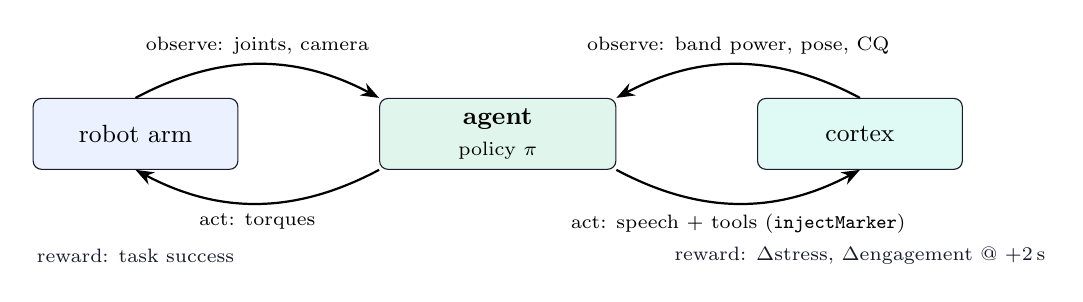
\begin{tikzpicture}[
  font=\small,
  box/.style={draw=ink, rounded corners=3pt, minimum height=9mm, minimum width=26mm, align=center},
  lab/.style={font=\scriptsize, midway},
  >=Stealth]
  \node[box, fill=agent!12, minimum width=30mm] (agent) at (0,0) {\textbf{agent}\\ \scriptsize policy $\pi$};
  \node[box, fill=alphac!15] (arm) at (-4.6,0) {robot arm};
  \node[box, fill=theta!18] (brain) at (4.6,0) {cortex};
  % left loop
  \draw[->, thick] (arm.north) to[bend left=28] node[lab, above]{observe: joints, camera} (agent.north west);
  \draw[->, thick] (agent.south west) to[bend left=28] node[lab, below]{act: torques} (arm.south);
  % right loop
  \draw[->, thick] (brain.north) to[bend right=28] node[lab, above]{observe: band power, pose, CQ} (agent.north east);
  \draw[->, thick] (agent.south east) to[bend right=28] node[lab, below]{act: speech + tools (\texttt{injectMarker})} (brain.south);
  % rewards
  \node[font=\scriptsize, text=ink] at (-4.6,-1.55) {reward: task success};
  \node[font=\scriptsize, text=ink] at (4.6,-1.55) {reward: $\Delta$stress, $\Delta$engagement @ +2\,s};
\end{tikzpicture}
\caption{One agent, two embodiments, one contract. The loops are structurally identical; only the sensors and actuators differ. The right-hand loop is what this paper builds.}
\label{fig:contract}
\end{figure}

Two honest asymmetries, before anyone objects. First, \emph{actuation is indirect}: the agent does not stimulate the cortex, it speaks to a person, and the person's brain responds. But indirection is not disqualifying --- a quadruped's policy does not command foot positions either; it commands motors and the ground responds. The contract requires an action channel with measurable consequences, and speech into a marked EEG record is exactly that. Second, \emph{the reward is slow and noisy}: cognitive metrics arrive at 0.1\,Hz, and Part II \S6 reports --- without cosmetics --- how often that leaves the reward undefined in a 12-second episode. Robot people will recognize this problem instantly. It is sparse reward, and their field has a decade of machinery for it. That is rather the point: once the contract holds, the machinery transfers.

% ==================================================================
\section{What Cortex actually gives you}
\label{sec:cortex}

Between the electrodes and our code sits EMOTIV's Cortex service~\cite{emotiv2024cortex}: a local WebSocket API (\texttt{wss://localhost:6868}) that owns the headset and hands out JSON streams by subscription. What you receive depends on your license, and papers rarely say what a \emph{consumer} setup really delivers. So we measured it. Table~\ref{tab:streams} and Figure~\ref{fig:rates} come from one 10-second live capture --- 865 samples, shipped in our test suite as a fixture, so every rate in this section is reproducible with \texttt{wc -l} and a stopwatch.\footnote{\texttt{tests/fixtures/epocx\_live\_10s.jsonl}. Counting lines by stream reproduces the table exactly.}

\begin{table}[h]
\centering
\small
\begin{tabular}{@{}llrrl@{}}
\toprule
\textbf{stream} & \textbf{carries} & \textbf{samples/10\,s} & \textbf{$\approx$Hz} & \textbf{what it is good for} \\
\midrule
\texttt{mot} & quaternion + accelerometer + magnetometer & 338 & 33.8 & deliberate gesture, $\sim$50\,ms \\
\texttt{fac} & eye action, upper/lower face + power & 337 & 33.7 & blinks, winks, clench --- buttons \\
\texttt{pow} & band power, 14 ch $\times$ 5 bands & 84 & 8.4 & the observation vector \\
\texttt{com} & trained mental command + power & 84 & 8.4 & one bit of consent \\
\texttt{dev} & contact quality per electrode, battery & 21 & 2.1 & whether to believe anything above \\
\texttt{met} & 7 cognitive metrics & 1 & 0.1 & mood over minutes, never moments \\
\midrule
\texttt{eeg} & raw waveform, 256\,Hz & \multicolumn{3}{l}{\emph{denied: error \texttt{-32016}, requires a paid license}} \\
\bottomrule
\end{tabular}
\caption{Everything a Basic (free) Cortex license delivers, measured over one live 10\,s capture (865 samples total). Raw EEG is refused, which forced a design honesty: \texttt{pow} at 8\,Hz is the observation, and 8\,Hz becomes the dataset frame rate in Part II.}
\label{tab:streams}
\end{table}

\begin{figure}[h]
\centering
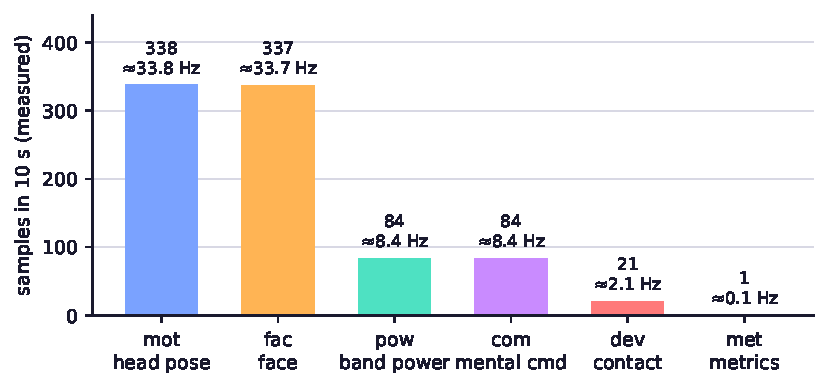
\includegraphics[width=0.82\linewidth]{stream_rates}
\caption{The same measurement, drawn. Motion and face dominate the wire ($\sim$34\,Hz each); the cognitive metrics everyone actually wants arrive \emph{once} in 10 seconds. Any design that pretends otherwise is fiction. Source: the 865-sample fixture.}
\label{fig:rates}
\end{figure}

Three consequences shaped everything downstream. \emph{First}, no raw EEG means no custom signal processing to brag about --- and no way to fool ourselves. Cortex's own band power is the observation, take it or leave it. \emph{Second}, the interesting streams are slow. Band power at 8\,Hz sets the heartbeat of the whole system; the dataset in Part II inherits \texttt{fps=8} directly from this table. \emph{Third}, the fast streams (\texttt{mot}, \texttt{fac} at $\sim$34\,Hz) are fast enough for something the slow streams can never do: reflexes. That split --- fast gesture, slow weather --- is not an implementation detail. It is the architecture, and it gets its own section.

One more measured caveat: the \texttt{met} vector nominally carries seven metrics, but \texttt{attention} is only present while Cortex's detector is active. Our rule, learned the hard way: \emph{nothing may gate on a metric that can be absent} (\S\ref{sec:ambient}).

% ==================================================================
\section{Three speeds, never mixed}
\label{sec:speeds}

A single control loop cannot serve a brain. Run it fast and the mood estimates jitter into noise; run it slow and a wink takes ten seconds to land. The system therefore listens at three speeds, and the rule that keeps it sane is that \emph{information never crosses between speeds implicitly} (Figure~\ref{fig:speeds}).

\begin{figure}[h]
\centering
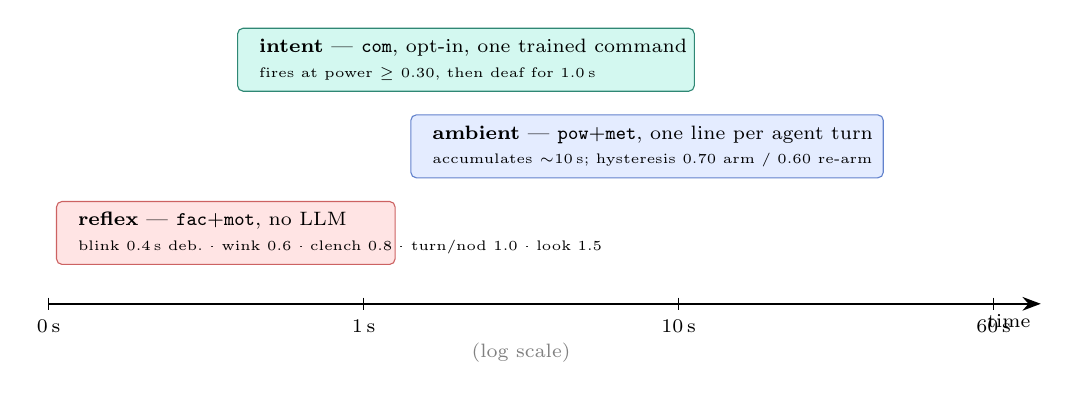
\begin{tikzpicture}[font=\small, >=Stealth]
  % time axis
  \draw[->, thick] (0,0) -- (12.6,0) node[below left, font=\scriptsize]{time};
  \foreach \x/\l in {0/0\,s, 4/1\,s, 8/10\,s, 12/60\,s}
    \draw (\x,0.08) -- (\x,-0.08) node[below, font=\scriptsize]{\l};
  \node[font=\scriptsize, gray] at (6,-0.62) {(log scale)};
  % reflex lane
  \draw[fill=betaH!20, draw=betaH!80!black, rounded corners=2pt] (0.1,0.5) rectangle (4.4,1.3);
  \node[anchor=west, font=\scriptsize] at (0.25,1.05) {\textbf{reflex} --- \texttt{fac}+\texttt{mot}, no LLM};
  \node[anchor=west, font=\tiny] at (0.25,0.72) {blink 0.4\,s deb.\ · wink 0.6 · clench 0.8 · turn/nod 1.0 · look 1.5};
  % ambient lane
  \draw[fill=alphac!20, draw=alphac!80!black, rounded corners=2pt] (4.6,1.6) rectangle (10.6,2.4);
  \node[anchor=west, font=\scriptsize] at (4.75,2.15) {\textbf{ambient} --- \texttt{pow}+\texttt{met}, one line per agent turn};
  \node[anchor=west, font=\tiny] at (4.75,1.82) {accumulates $\sim$10\,s; hysteresis 0.70 arm / 0.60 re-arm};
  % intent lane
  \draw[fill=theta!25, draw=theta!60!black, rounded corners=2pt] (2.4,2.7) rectangle (8.2,3.5);
  \node[anchor=west, font=\scriptsize] at (2.55,3.25) {\textbf{intent} --- \texttt{com}, opt-in, one trained command};
  \node[anchor=west, font=\tiny] at (2.55,2.92) {fires at power $\ge$ 0.30, then deaf for 1.0\,s};
\end{tikzpicture}
\caption{The three listening speeds and where they live on the clock. Every constant is quoted from \texttt{events.py}; none are illustrative. Reflex acts without a model; ambient only colors the agent's next turn; intent is a single bit reserved for consent (\S\ref{sec:consent}).}
\label{fig:speeds}
\end{figure}

\textbf{Reflex} ($\le$100\,ms, no language model in the loop). Deliberate face and head gestures become discrete events: blink, double blink, wink left/right, clench, head turn left/right, nod, look up/down. Each has a debounce --- a minimum silence between firings of the same kind --- taken verbatim from the code: blink 0.4\,s, winks 0.6\,s, clench 0.8\,s, turns and nods 1.0\,s, looks 1.5\,s; a second blink within 0.8\,s upgrades to \texttt{double\_blink}. Head gestures come from the quaternion: a yaw excursion of $\ge$20$^\circ$ inside one second is a turn; a pitch dip of $\ge$10$^\circ$ that returns to within 5$^\circ$ of baseline inside 1.5\,s is a nod. Figure~\ref{fig:headpose} shows the raw material: ten seconds of live head pose with the turn threshold drawn to scale --- ordinary stillness stays an order of magnitude under it, which is exactly why a threshold this size reads \emph{deliberateness}.

\begin{figure}[h]
\centering
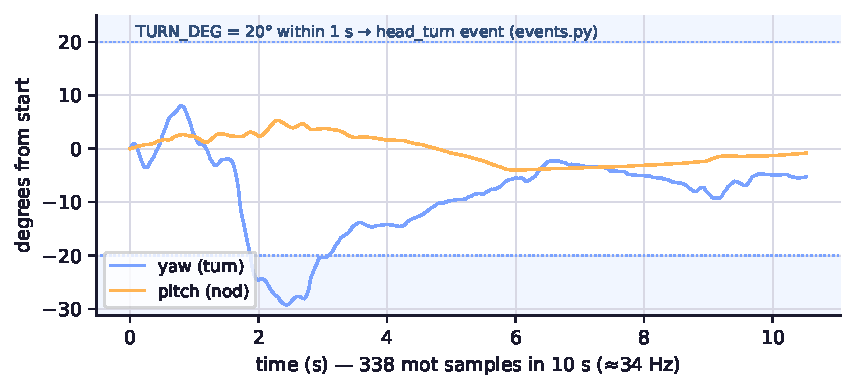
\includegraphics[width=0.85\linewidth]{headpose}
\caption{Ten live seconds of head pose, decoded from the \texttt{mot} quaternion (338 samples). The shaded region is the turn threshold (20$^\circ$ within 1\,s). A resting head never grazes it; a deliberate turn crosses it in a few hundred milliseconds. Source: the same 10\,s fixture as Table~\ref{tab:streams}.}
\label{fig:headpose}
\end{figure}

\textbf{Ambient} ($\sim$10\,s). Band power and metrics accumulate into the one-line summary of \S\ref{sec:ambient}. Slow-lane threshold events (focus high, stress high) use hysteresis rather than debounce: \emph{focus\_high} arms at 0.70 and cannot fire again until the metric falls below 0.60. A value oscillating around a threshold therefore produces one event, not a drumroll.

\textbf{Intent} (opt-in). One trained mental command --- \emph{push} --- fires only above power 0.30 and then goes deaf for a full second. It carries exactly one bit, and that bit is reserved for consent.

The never-mix rule earns its keep in the failure cases. A blink must not nudge the mood estimate (it is a motor artifact, not affect). A stressful minute must not make the blink detector trigger-happy (thresholds are constants, not moods). And the mental command must not become a steering wheel --- the moment ``push'' means more than \emph{yes}, the user is back to operating a machine instead of talking to something that listens.

% ==================================================================
\section{The ambient line}
\label{sec:ambient}

Everything the slow streams know is compressed into one line of text, prepended to every agent turn:

\begin{center}
\colorbox{ink!4}{\texttt{[brain: focus 0.71 · stress 0.22 · alpha dominant O1/O2 · CQ 13/14 good]}}
\end{center}

That line is the whole interface between your nervous system and the language model, so its anatomy deserves a paragraph. It is assembled in a fixed order by one function (\texttt{ambient\_line()} in \texttt{tools.py}). First the metrics that are \emph{present}: focus, stress, engagement, each as a bare number --- the agent is told ``your focus metric fell,'' never ``you're bored''; the number stays a number. Then the dominant band across all 14 channels, tagged with O1/O2 when alpha wins there --- occipital alpha being the classic eyes-closed, mind-idling signature~\cite{klimesch1999alpha}. Then the last reflex event, if any. Last, always, the contact-quality fraction.

Two rules give the line its integrity:

\textbf{Absent is not zero.} On a Basic license the \texttt{attention} metric only exists while Cortex's detector happens to run (\S\ref{sec:cortex}). A naive formatter would print \texttt{focus 0.00} and the agent would conclude the user is comatose. Ours prints nothing: a missing metric vanishes from the line, and the schema in Part II carries an explicit validity mask for the same reason. The difference between $0$ and $\varnothing$ is the difference between a measurement and a lie.

\textbf{Contact quality gates everything.} The line opens with brain facts only if overall contact quality clears $0.5$ (\texttt{CQ\_USABLE}); an electrode counts as good at quality $\ge$3 of 4. Below the gate the entire line collapses to \texttt{[brain: not visible: contact quality too low]} and the agent says so and behaves as a plain assistant. No degraded guessing, no confident readings from dry electrodes. Figure~\ref{fig:cq} shows the fraction that backs the \texttt{13/14} in the example line --- one temporal electrode sitting slightly proud of the scalp for the whole session, honestly reported, correctly ignored.

\begin{figure}[h]
\centering
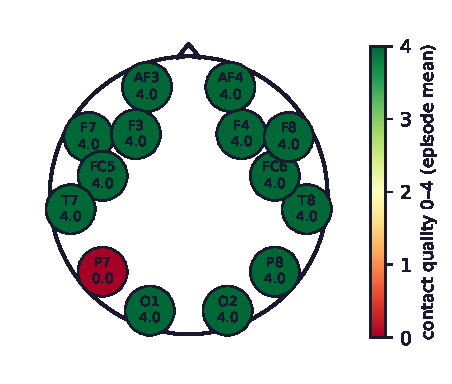
\includegraphics[width=0.5\linewidth]{cq_map}
\caption{Contact quality on the 10--20 montage~\cite{jasper1958ten}, episode mean over the 99 frames of \texttt{live-accept-1}. Thirteen electrodes at full quality; T8 partial. This map is why the ambient line ends in \texttt{CQ 13/14}: the agent's confidence in every number to its left is anchored by the fraction on its right.}
\label{fig:cq}
\end{figure}

The compression is the point. We could hand the model 70 floats per frame; it would produce horoscopes. One line, engineered from measured quantities, with absence preserved and a trust score attached, turns out to be what a language model can actually \emph{use}: stress reads high and answers get shorter; a thinking pause gets silence instead of a follow-up question. The friend across the table does not recite your vitals either. They notice, and it changes their tone.

% ==================================================================
\section{The mirror}
\label{sec:mirror}

We did not design this system in a document. We designed it in a dashboard, with the headset on, watching. The layout is a sentence you can read (Figure~\ref{fig:dashboard}): \emph{left, you; right, the agent; bottom, the conversation.} The left column is the body --- live band scope, the $\theta$--$\gamma$ radar, the CQ-colored head map, head pose, metric gauges, an event ticker. The right column is the machine's mind: the exact ambient line the agent will read next turn, the last reflex event it caught, the last marker it stamped. You watch the agent watching you.

\begin{figure}[h]
\centering
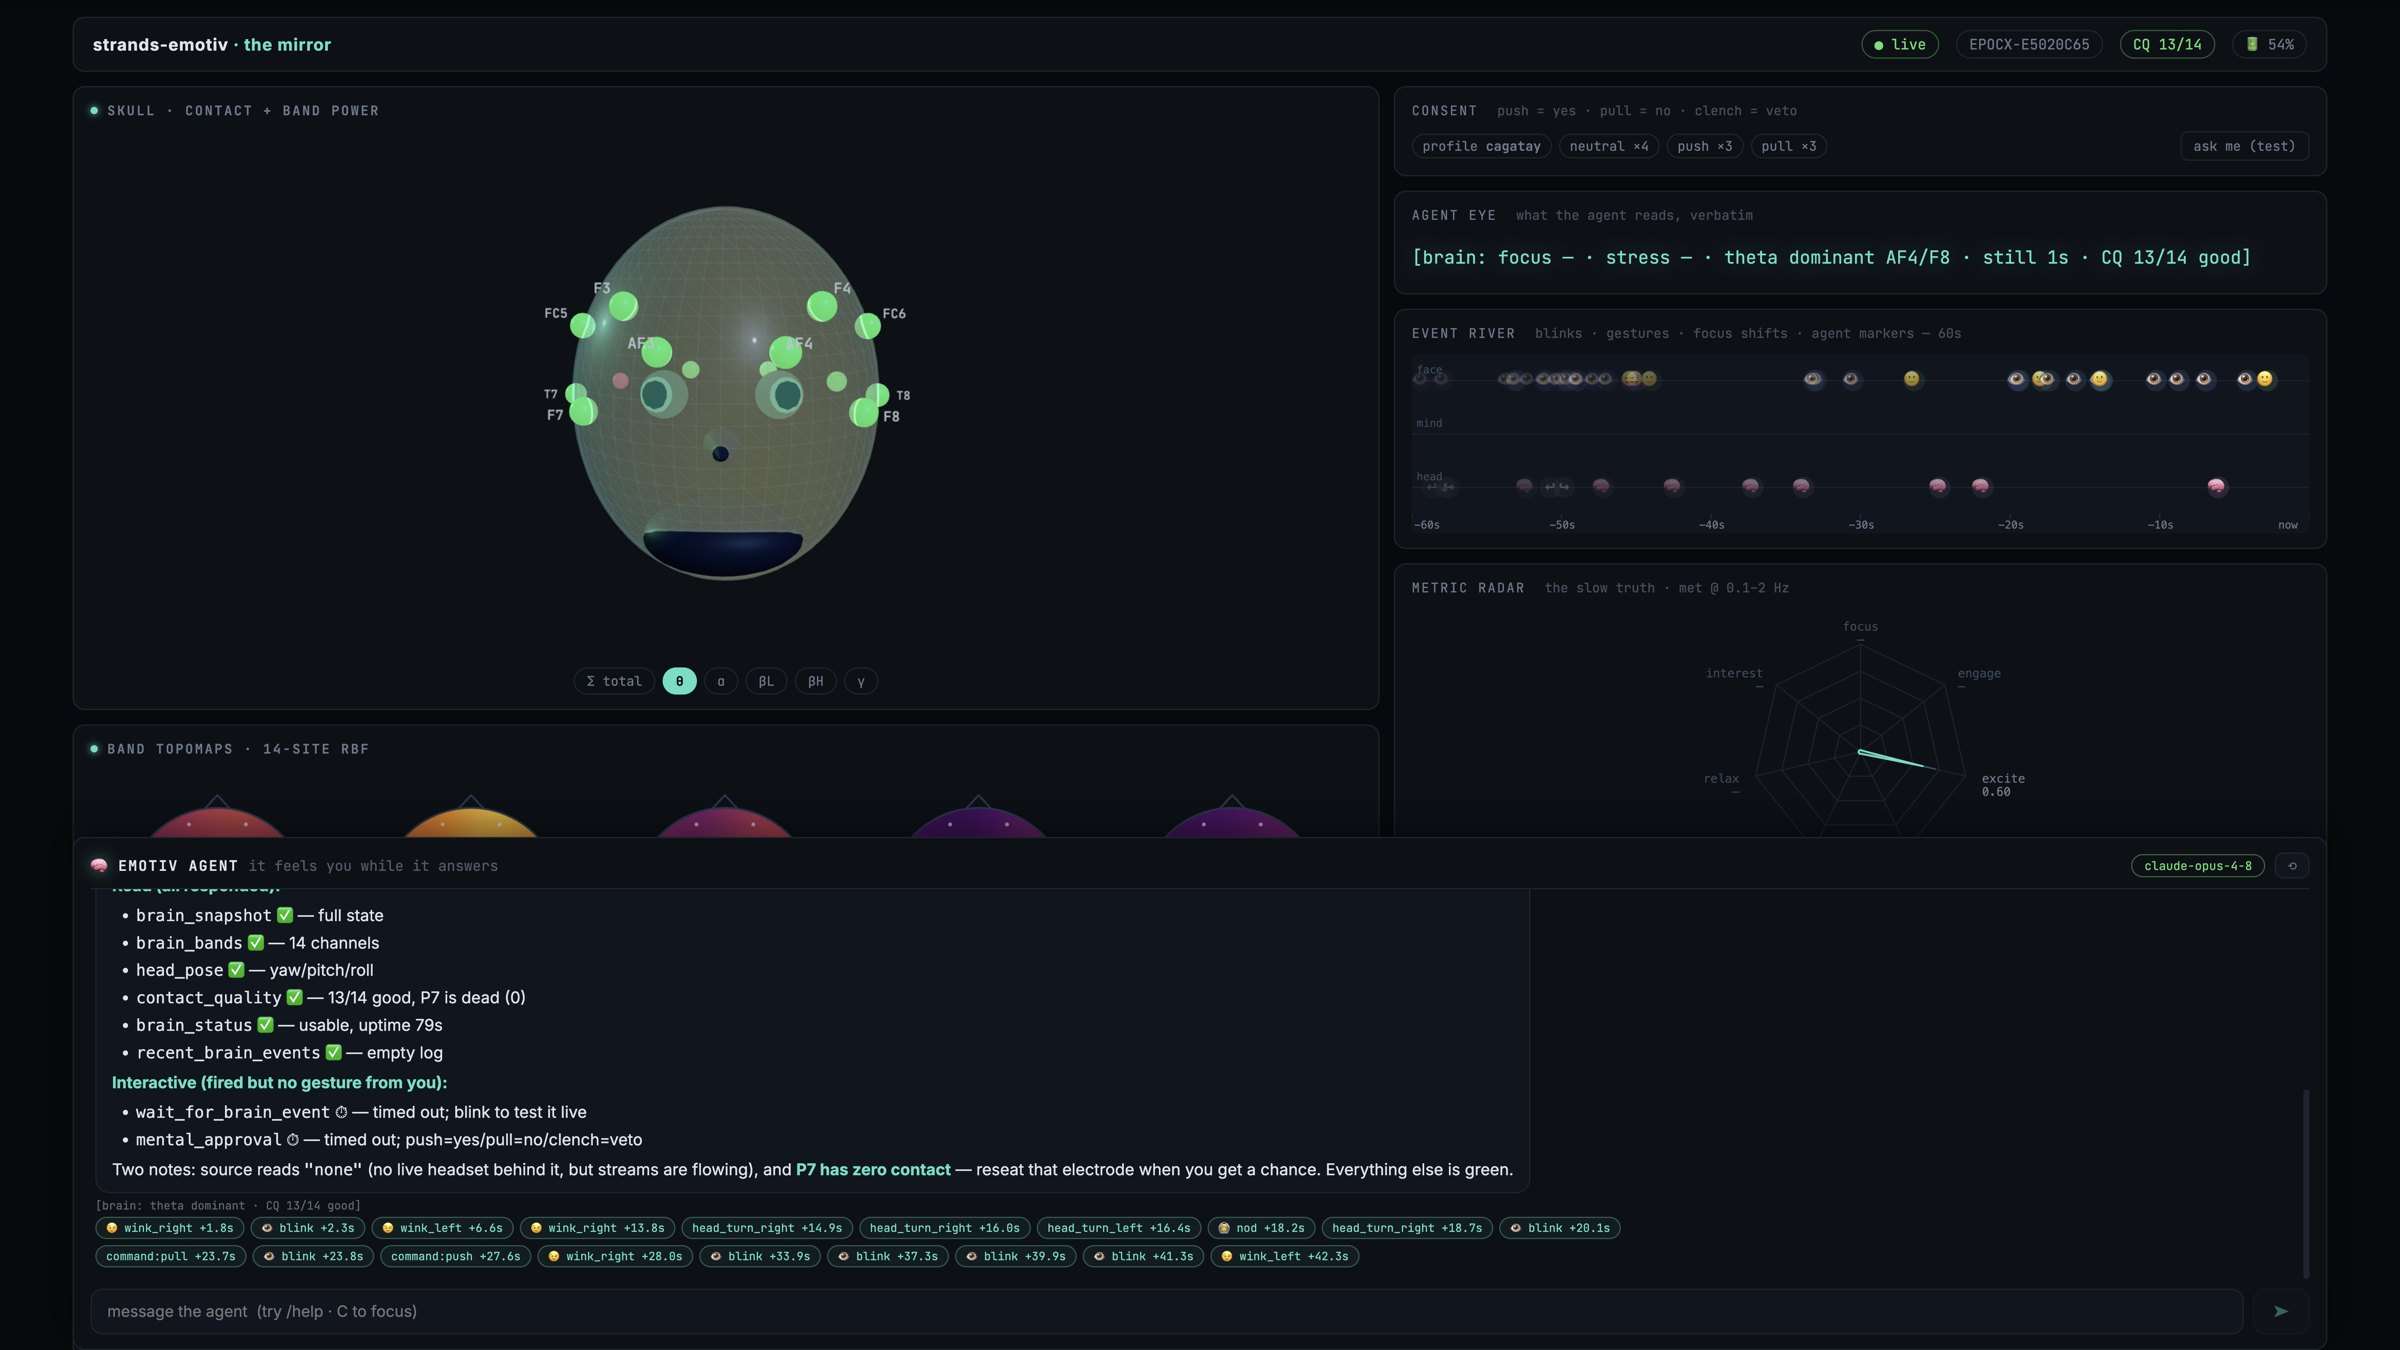
\includegraphics[width=0.95\linewidth]{dashboard.jpg}
\caption{The mirror, live. Left column: the body (band scope, radar, 10--20 head map colored by contact quality, head pose, gauges). Right column: the agent (the ambient line verbatim, last event, last marker, consent panel). Bottom: chat. Photo from a live session (\texttt{docs/img/dashboard.jpg}).}
\label{fig:dashboard}
\end{figure}

Calling it a \emph{mirror} is precise, not poetic. The dashboard renders the identical string the model receives --- not a prettier cousin of it --- so every design failure becomes visible in seconds. This is how the three-speeds rule was actually discovered: an early build fed blinks into the mood estimate, the radar twitched with every blink, and the lie was on screen before it could calcify into architecture. The hysteresis constants of \S\ref{sec:speeds} were tuned the same way --- watching \emph{focus\_high} drumroll around its threshold until the arm/re-arm gap silenced it.

\begin{figure}[h]
\centering
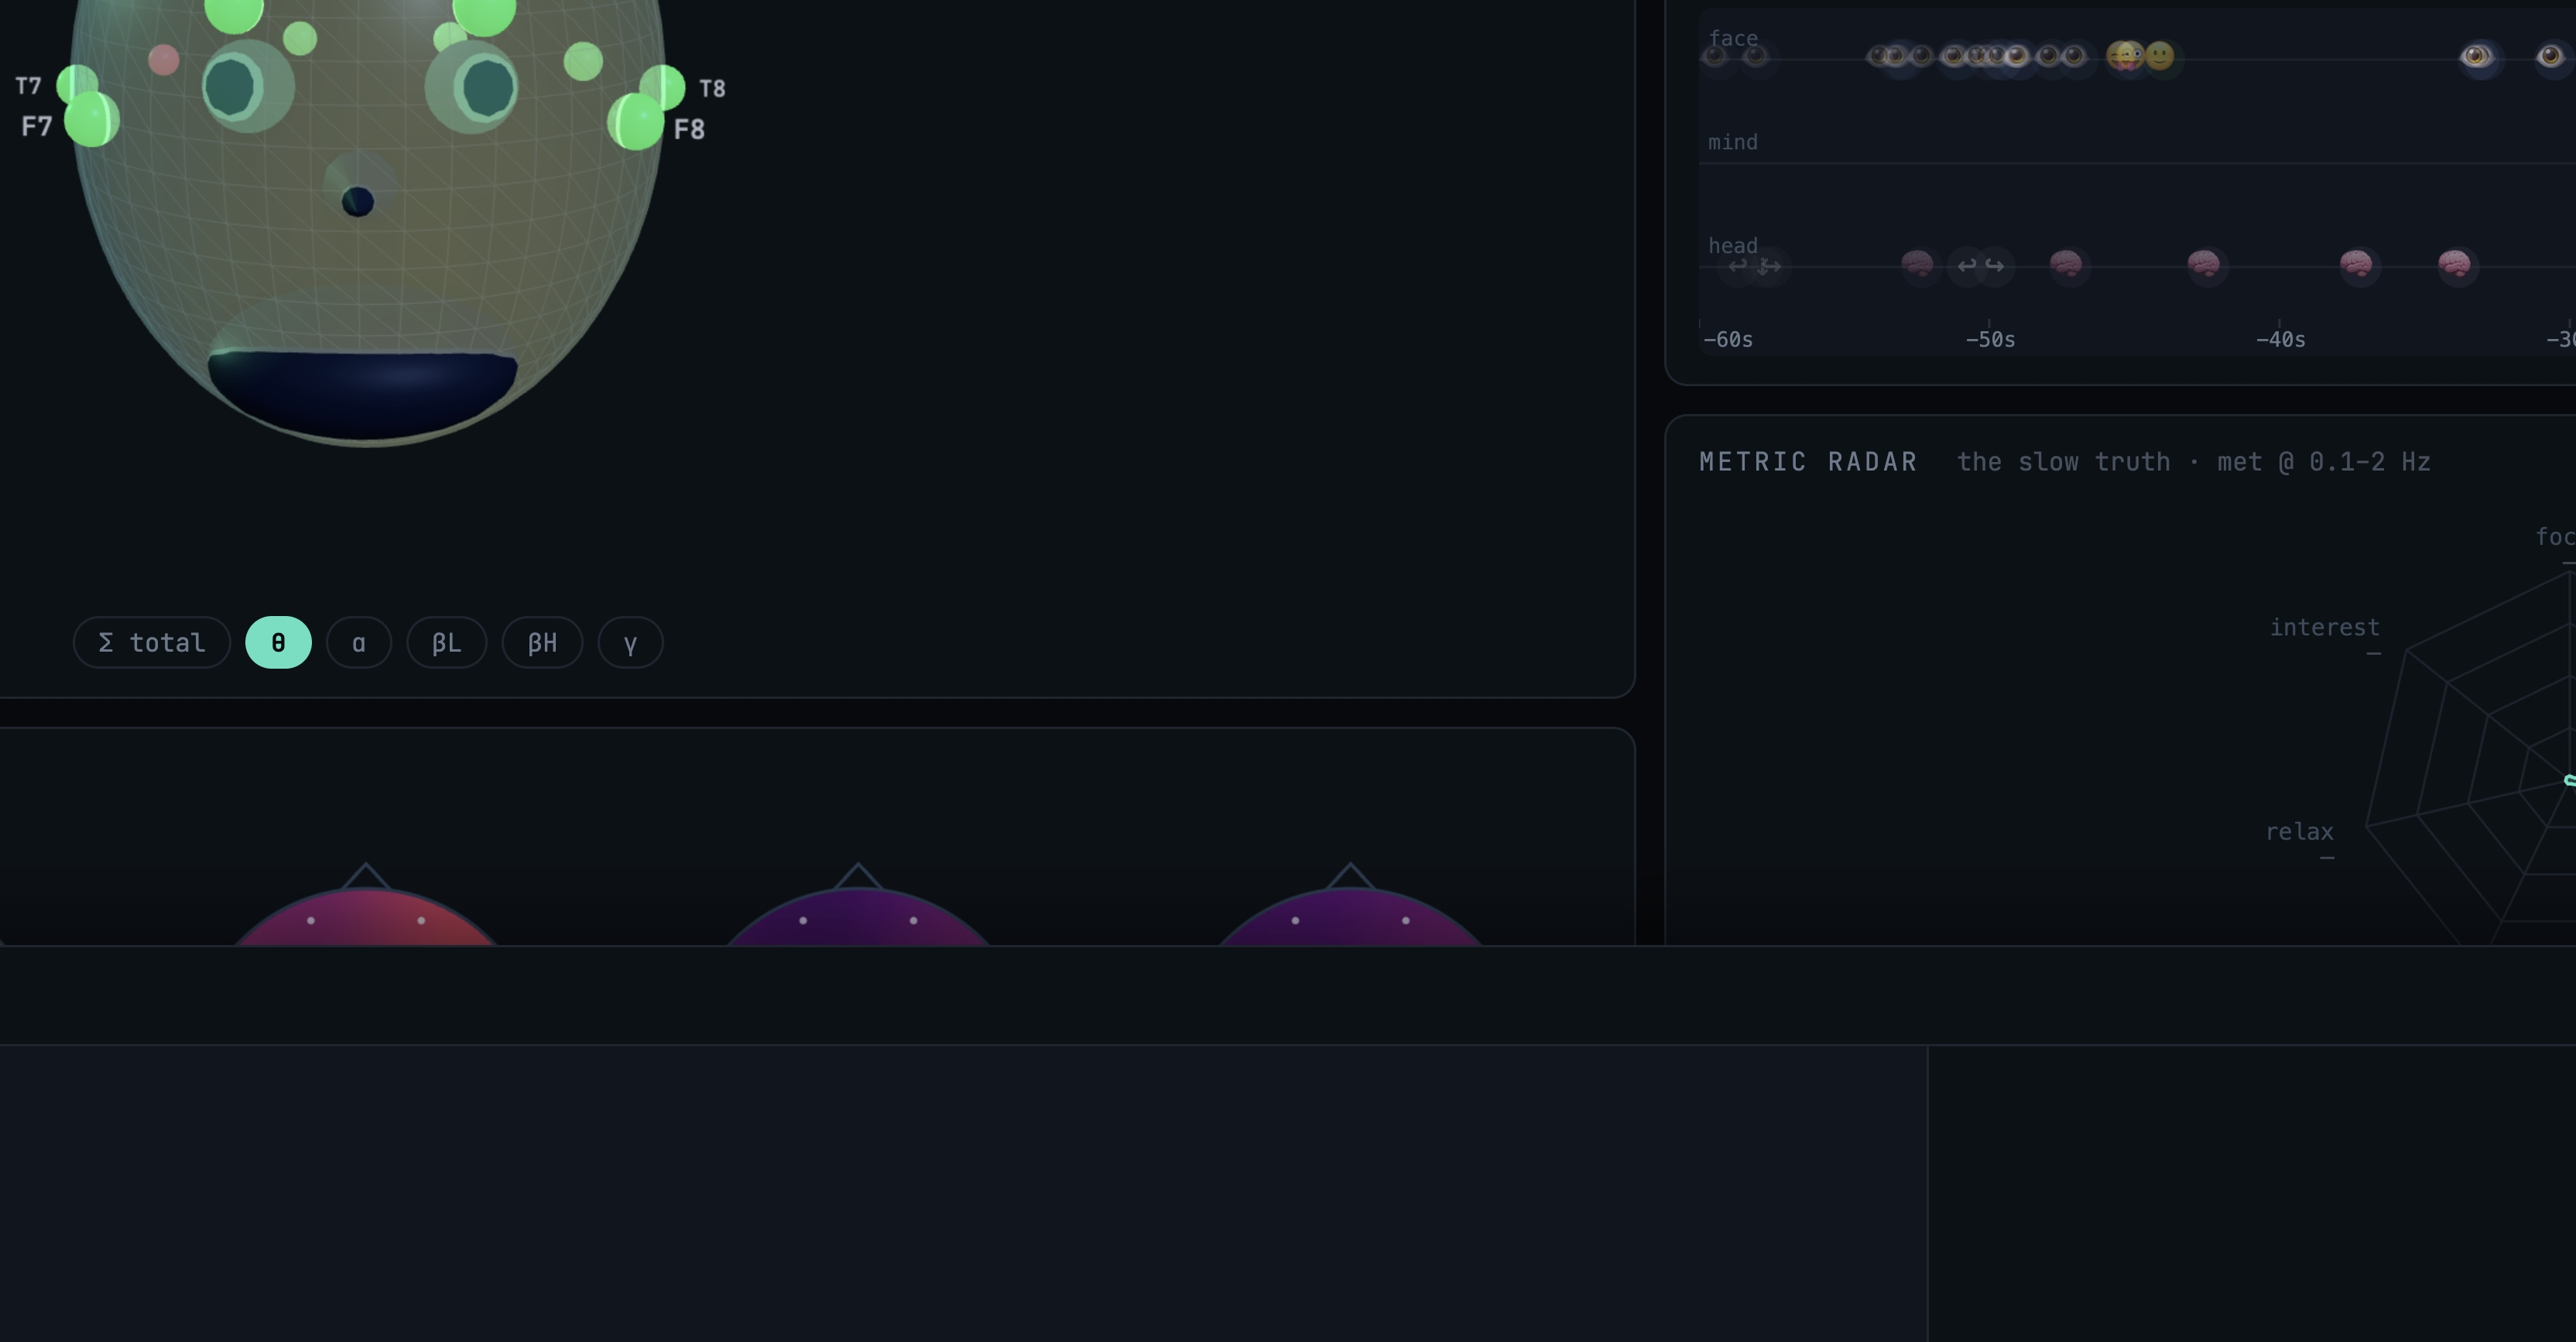
\includegraphics[width=0.95\linewidth]{topomaps-waterfall.jpg}
\caption{The slow weather, two ways: per-band scalp topomaps ($\theta$ through $\gamma$) above the rolling band-power waterfall. The waterfall's vertical stripes are the session's history; the topomaps are its present tense. Photo from the same live session (\texttt{docs/img/topomaps-waterfall.jpg}).}
\label{fig:topomaps}
\end{figure}

An instrument like this changes who can do the work. Every threshold in this paper was set by the person wearing the headset, in conversation with the agent being tuned, both looking at the same pixels. When the wearer says ``that wasn't a nod'' and the ticker disagrees, the constant is wrong and everyone present knows it immediately. We recommend the practice to anyone building on bodies they do not inhabit.

% ==================================================================
\section{Consent as the only command}
\label{sec:consent}

The 2019 project's entire ambition --- mind as controller --- survives here as exactly one bit. The user may train a single Cortex mental command, \emph{push}: imagine pushing a box away from you. When the agent needs permission for something consequential, it asks, and the dashboard's consent panel opens a countdown. Push means \emph{yes}. A trained \emph{pull} means \emph{no}. And a jaw clench --- a reflex-lane event, no model in the loop, debounced at 0.8\,s --- is an unconditional veto at any layer, at any time, including mid-answer.

The asymmetry is deliberate. Assent rides the slowest, most deliberate channel we have (a trained mental image held above power 0.30, \S\ref{sec:speeds}); refusal rides the fastest (a muscle). Saying \emph{yes} to an agent should take effort; saying \emph{stop} should not even require intent to be legible. Anything the agent does can be interrupted by a gesture that costs nothing and cannot be misread --- \texttt{clench} maps to \emph{cancel everything} at every layer, unconditionally.

This is also why \emph{push} is reserved for consent and never steering (\S\ref{sec:speeds}). A steering wheel made of imagination is the slower keyboard of \S\ref{sec:joystick} all over again. A consent channel made of imagination is something a keyboard cannot be: proof the user meant it, on the same clock, in the same record, as the brain that meant it.

% ==================================================================
\section{System}
\label{sec:system}

The whole apparatus is one Python package, one WebSocket session, and one page (Figure~\ref{fig:arch}). Cortex owns the headset; we own everything after the socket.

\begin{figure}[h]
\centering
\resizebox{\linewidth}{!}{%
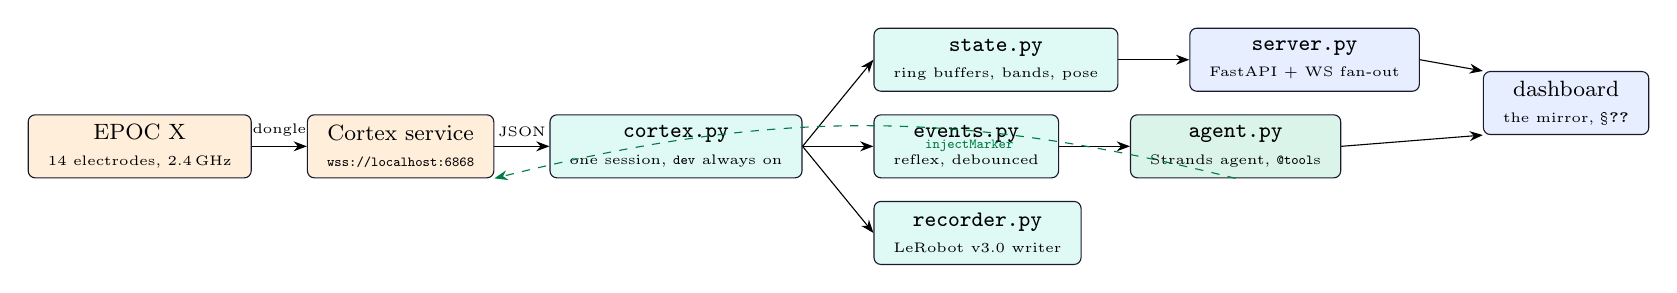
\begin{tikzpicture}[
  font=\small, >=Stealth, node distance=4mm,
  mod/.style={draw=ink, rounded corners=2.5pt, minimum height=8mm, align=center, font=\footnotesize, inner xsep=2.5mm},
  hw/.style={mod, fill=betaL!22},
  core/.style={mod, fill=theta!18},
  face/.style={mod, fill=alphac!18},
  ag/.style={mod, fill=agent!14}]
  \node[hw] (headset) {EPOC X\\ \tiny 14 electrodes, 2.4\,GHz};
  \node[hw, right=7mm of headset] (cortex) {Cortex service\\ \tiny \texttt{wss://localhost:6868}};
  \node[core, right=7mm of cortex] (client) {\texttt{cortex.py}\\ \tiny one session, \texttt{dev} always on};
  \node[core, right=9mm of client, yshift=11mm] (state) {\texttt{state.py}\\ \tiny ring buffers, bands, pose};
  \node[core, right=9mm of client] (events) {\texttt{events.py}\\ \tiny reflex, debounced};
  \node[core, right=9mm of client, yshift=-11mm] (recorder) {\texttt{recorder.py}\\ \tiny LeRobot v3.0 writer};
  \node[face, right=9mm of state] (server) {\texttt{server.py}\\ \tiny FastAPI + WS fan-out};
  \node[ag, right=9mm of events] (agent) {\texttt{agent.py}\\ \tiny Strands agent, \texttt{@tool}s};
  \node[face, right=8mm of server, yshift=-5.5mm] (dash) {dashboard\\ \tiny the mirror, \S\ref{sec:mirror}};
  \draw[->] (headset) -- node[above, font=\tiny]{dongle} (cortex);
  \draw[->] (cortex) -- node[above, font=\tiny]{JSON} (client);
  \draw[->] (client.east) -- (state.west);
  \draw[->] (client.east) -- (events.west);
  \draw[->] (client.east) -- (recorder.west);
  \draw[->] (state.east) -- (server.west);
  \draw[->] (events.east) -- (agent.west);
  \draw[->] (server.east) -- (dash.north west);
  \draw[->] (agent.east) -- (dash.south west);
  \draw[->, dashed, agent!70!black] (agent.south) to[bend right=14] node[below, font=\tiny, pos=0.35]{\texttt{injectMarker}} (cortex.south east);
\end{tikzpicture}}
\caption{One session, three consumers. \texttt{cortex.py} holds the only Cortex connection and always co-subscribes \texttt{dev}, so no consumer can ever see brain data without its contact quality. State, events, and the recorder fan out from the same bus; the agent's actions flow back into the EEG record through \texttt{injectMarker} (dashed) --- the arrow that makes Part II possible.}
\label{fig:arch}
\end{figure}

Some load-bearing choices, briefly. \emph{One session}: Cortex permits one app session per headset, so a single client (\texttt{cortex.py}) owns it and everything else subscribes to an internal bus --- the dashboard, the agent, and the dataset recorder are peers reading one stream of truth. \emph{\texttt{dev} always co-subscribed}: contact quality is not optional telemetry; it rides along with every subscription so the gate of \S\ref{sec:ambient} can never be starved. \emph{Fixtures are first-class}: the same bus replays the 865-sample capture of \S\ref{sec:cortex}, so the full stack --- events, ambient line, recorder --- runs headless in CI. The test suite is 115 tests and covers the debounce and hysteresis behavior of \S\ref{sec:speeds} against recorded, not synthetic, samples.\footnote{Repo state at commit \texttt{b772395}: 115 passed. The suite replays \texttt{tests/fixtures/} through the same code path live data takes.} \emph{Remote access is a passkey, not a password}: the dashboard is public behind WebAuthn~\cite{webauthn2021}; brain streams deserve at least the security of a bank login. And the agent side is deliberately boring: a stock Strands agent~\cite{strands2025sdk} whose only specialness is its toolbox --- \texttt{brain\_snapshot}, \texttt{brain\_bands}, \texttt{mental\_approval}, \texttt{record\_start/stop} --- plus the ambient line in its context. Boring is the result: the thesis needs the \emph{agent} to be replaceable.

% ==================================================================
\section{Limitations, honestly}
\label{sec:limits}

\textbf{This is one brain.} Every constant, plot, and episode in both papers comes from a single subject --- the first author --- over sessions on consecutive days. Nothing here is a population claim. The claim is architectural: the contract holds. Whether the thresholds transfer across people is future work, and we suspect several will not (the nod detector already flirts with this subject's habit of looking down at a keyboard).

\textbf{The observation is what Cortex says it is.} On a Basic license we receive band power, metrics, and detections computed inside a closed SDK~\cite{emotiv2024cortex}. We cannot audit the DSP; raw EEG is refused (\texttt{-32016}, \S\ref{sec:cortex}). We chose to treat Cortex the way roboticists treat a motor controller --- a trusted black box with a spec sheet --- but the reader should know the box is closed.

\textbf{Consumer electrodes drift.} Saline pads dry over a session; T8 spent an entire recording at partial quality (Figure~\ref{fig:cq}). The system is built to \emph{report} this rather than hide it, but reporting a weakness is not the same as not having it.

\textbf{The reward is thin.} Metrics at 0.1\,Hz mean a 12-second episode may contain zero fresh \texttt{met} samples; Part II \S6 quantifies exactly how often, and the $\Delta$stress/$\Delta$engagement reward is honestly \texttt{nan} in those windows. We did not paper over this with interpolation, and we make no claim that the recorded rewards are yet sufficient to train on.

\textbf{Affect is not thought.} Nothing in this system reads content. Band power and slow metrics are weather, not language --- closer to posture than to speech~\cite{picard1997affective}. Both the power and the safety of the design come from that ceiling, and we state it as a boundary, not an apology.

% ==================================================================
\section{Toward Part II}
\label{sec:towards}

Part I ends where most interaction papers end: a working system, a person wearing it, an agent that behaves differently because of it. But the embodiment contract of \S\ref{sec:contract} has a sharper test than ``it works.'' If the brain really is another embodiment, then its sessions should be \emph{robot data} --- storable in a robot dataset format, loadable by a robot data loader, annotated with the same chain-of-thought structure a manipulation policy trains on, with the reward living in the observation stream itself.

That test is pass/fail, and it runs in Part II: every conversational turn becomes a LeRobot v3.0 episode (3\,s of brain before the agent speaks, the marked action, the tail after); every frame carries an embodied chain-of-thought string in the dataset's task table; and an unmodified \texttt{LeRobotDataset} pulls \texttt{cagataydev/emotiv-ecot} from the HuggingFace Hub exactly as it would pull a manipulation corpus. The brain rides the same rails as every robot~\cite{cadene2024lerobot,zawalski2024ecot}.

\vspace{2mm}
\noindent\emph{Part II: ``Embodied Chain-of-Thought for a Cortex --- the Brain as Observation and Reward.''}

\bibliographystyle{unsrtnat}
\bibliography{../common/references}
\end{document}
